\documentclass[a4paper, titlepage]{jsarticle}

\date{\today}
\usepackage[dvipdfmx]{graphicx}
\usepackage{url}
% \usepackage[T1]{fontenc}
\usepackage{float}
\usepackage{ascmac}
\usepackage{pdfpages}
\usepackage{enumitem}

\title{ドローン宅配事業者支援システム}

\author{土佐山田IT株式会社 \and
  久保田 天治 \and 塩澤 康志 \and 蝉 祐介 \and 寺内 俊輔 \and 林 晃太郎 \and 松本 吏司}

\begin{document}
\maketitle

\tableofcontents

\clearpage

\section{現状の課題}
2022年日本における宅配便取扱個数は50億個を超えた.
忙しい日常がある中で,商品や郵便物を手軽に送受できる宅配便は多くの人々にとって頼りにされ,図\ref{fig:home_delivery}のように宅配需要は増加し続けている.
特に新型コロナウイルスの影響により,オンラインショッピングの増加や非接触配達の需要が高まり,宅配業界は一層の成長を遂げた.

しかし,宅配サービスの拡大と需要増加には新たな課題も浮かび上がっている,最も顕著な課題は宅配業界における労働力不足だ.
図\ref{fig:working_population}のように少子高齢化社会に伴う労働人口の減少により,現状の宅配サービスを維持することは日々困難になっている.
特に過疎地域や離島においては,現状の輸送方法では効率が悪く輸送方法の効率化が求められる.
\begin{figure}[H]
  \centering
  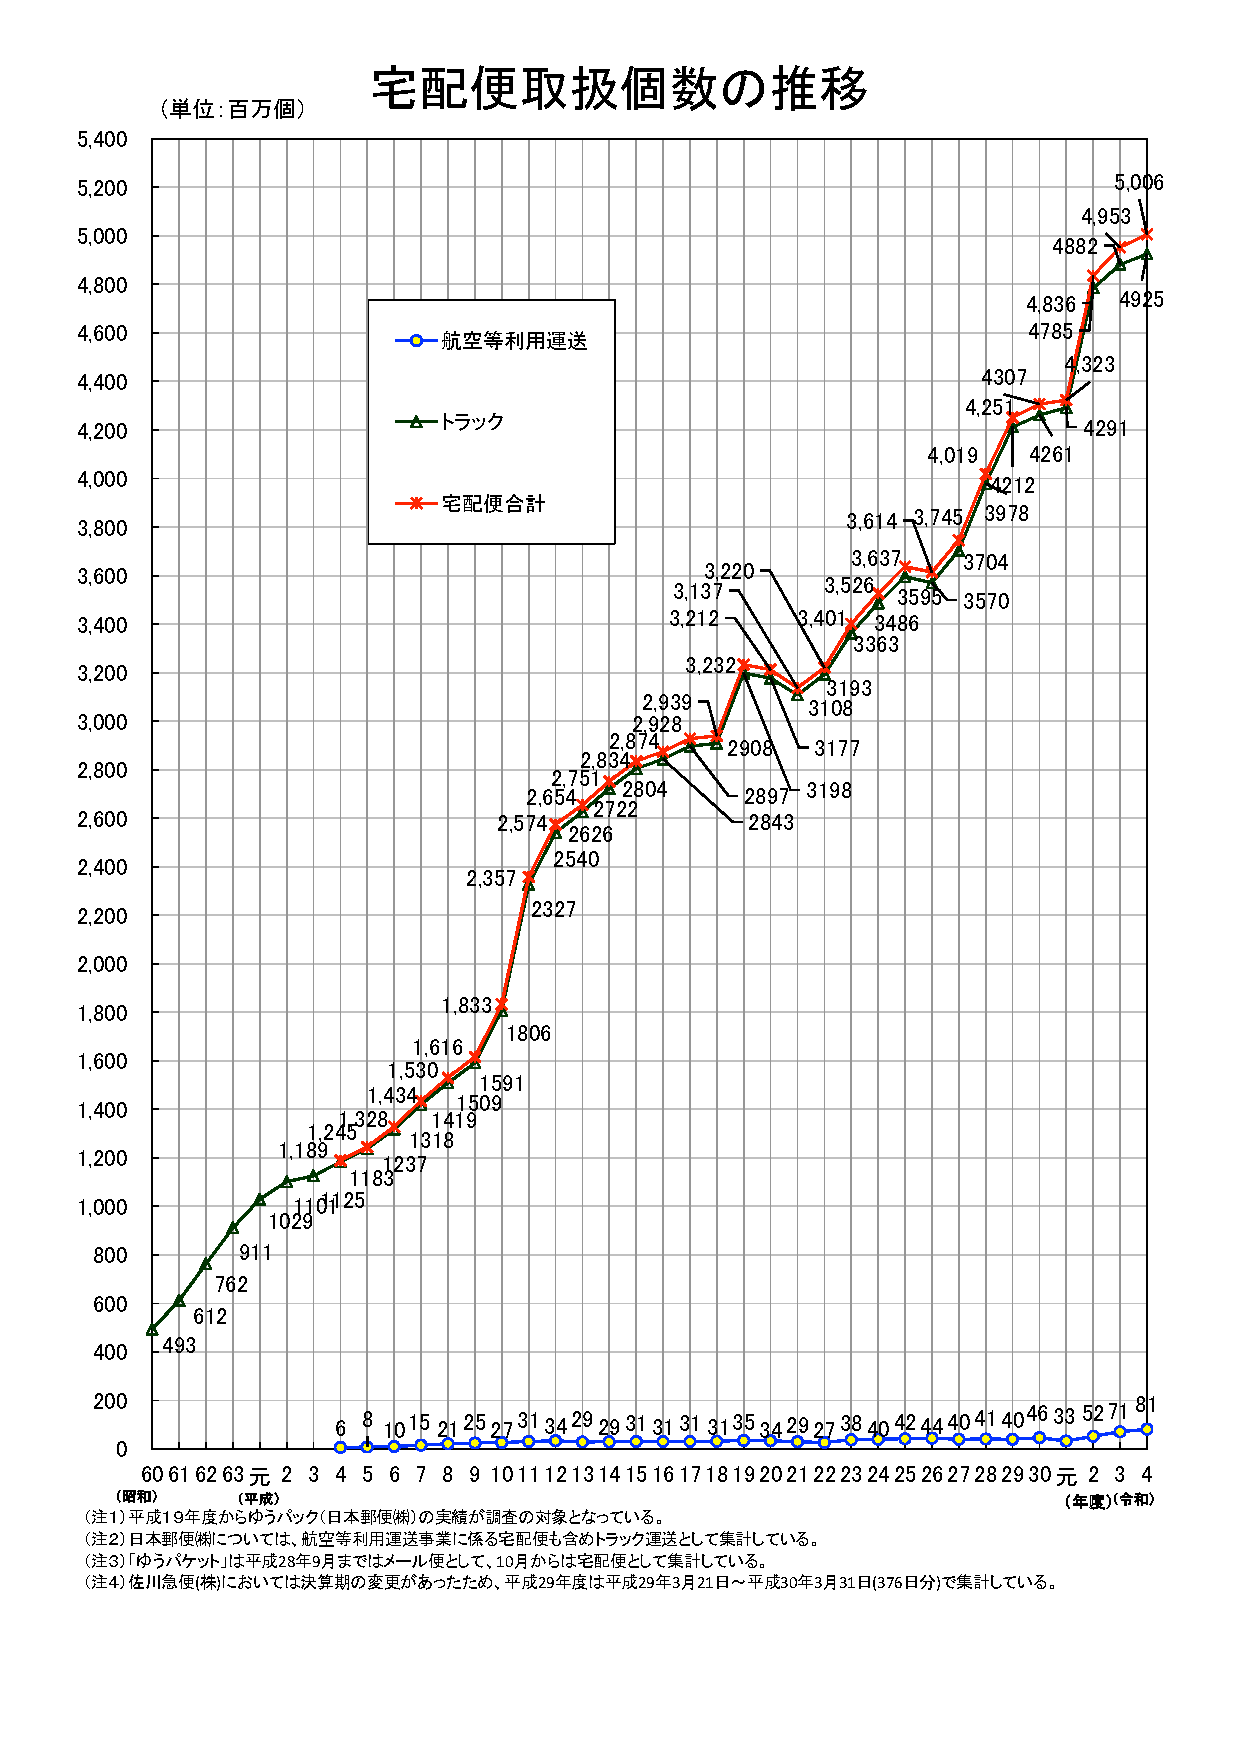
\includegraphics[width=0.6\textwidth]{./home_delivery.pdf}
  \caption{宅配便取扱個数の推移:\cite{home_delivery_2022}より引用}
  \label{fig:home_delivery}
\end{figure}
\begin{figure}[H]
  \centering
  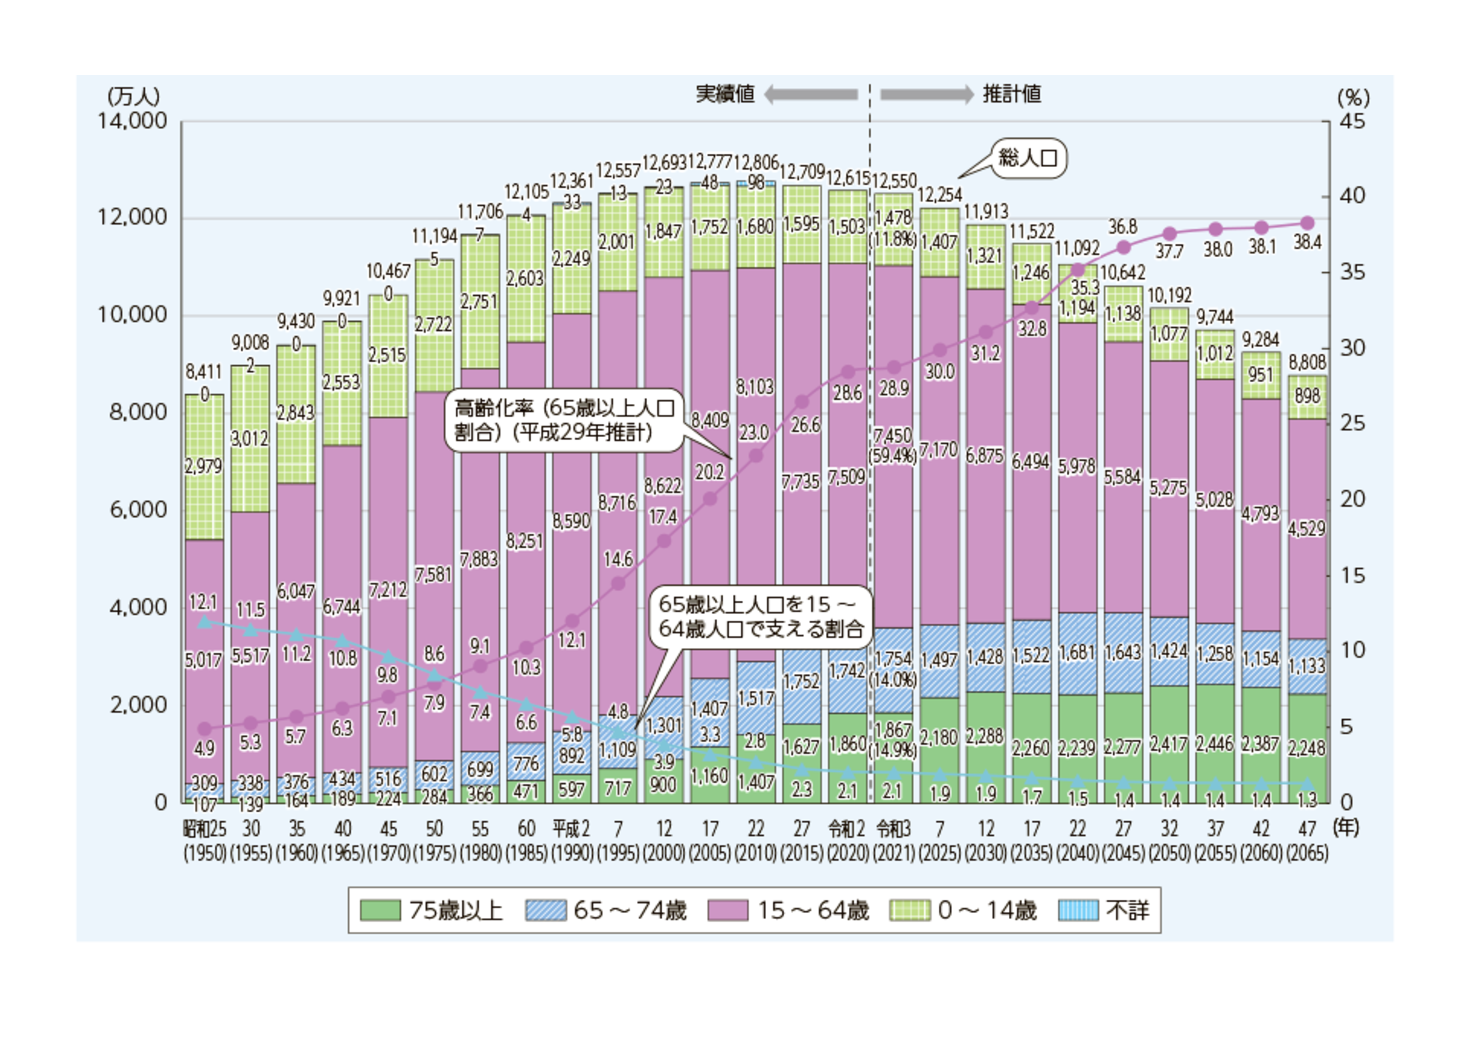
\includegraphics[width=0.8\textwidth]{./working_population.pdf}
  \caption{労働人口の減少:\cite{working_population_2022}より引用}
  \label{fig:working_population}
\end{figure}

\section{課題解決のための提案}
上記の課題を解決するため,効率的かつ人手不足を解消できるようなドローン宅配事業者支援システムを提案する.
このシステムによる課題の解決方法を以下に示す.
\begin{itemize}
  \item ドローンの操縦を自動化することで,より少ない人手で大量の荷物を個人宅に運搬でき,
        労働力不足の問題に対処できる.従来の宅配サービスと比較して労働者への依存度が低くなり,配送コスト削減と労働環境の改善に期待できる.

  \item 離島や過疎地域など従来の方法では配送コストが高かった地域にも,効率的に配送を行うことができる.
        これによりこれらの地域においても高速かつ手頃値段の宅配サービスが提供され,地域経済の活性化が促進できる.

  \item ドローン宅配事業者の支援システムは,多くの事業者に提供され新規ドローン宅配事業者の参入を奨励できる.
        新規ドローン宅配事業者の参入に伴う宅配業務従事者の増加と競争の活発化は,労働力不足の解消,サービス品質の向上,価格競争力の向上につながり,消費者にとって選択肢が増えることで市場が活性化する.

  \item 多くのドローン宅配事業者が共通の支援システムを使用することで,スケールメリットを最大限に活用しコスト削減を実現できる.
        経済的なメリットは宅配業界全体に波及し,より効率的なサービス提供が可能になる.

        % 本筋から外れるためコメントアウト
        % \item ドローン宅配は過疎地域の経済を支え,郊外地域に新たなビジネス機会を提供する.
        % 地域社会の発展に寄与し,地方経済を活性化させるポテンシャルがある.

        % \item 環境への負荷を軽減する.電動または電池駆動のドローンを使用することで,排ガス排出が削減され,環境への負荷が低減する.これは環境への配慮を重視する現代社会に貢献できる.
\end{itemize}

\section{ドローン宅配の実現可能性}
\subsection{ドローンとは}
ドローンとは,リモートコントロールや事前にプログラムされた自律システムによって飛行する小型の航空機であり,一般的には無人航空機とも呼ばれる.

ドローンは,手のひらに収まるほどの小型機から,長時間の飛行が可能な大型機まで,様々な種類がある.これらのドローンは,サイズ,形状,機能,価格などが多様であり,カメラ・センサー・GPS・通信機能などの多彩な機能を備えたモデルが存在している.

\subsection{ドローンに関する法律}
\begin{quote}
  ドローン物流サービスの提供にあたっては、飛行の安全の確保の観点から、航空法第 11 章無人航空機に掲げる規定を遵守する必要がある。遵守されていない場合、航空法第 13 章罰則に掲げる規定により、罪に問われる場合がある。(\cite{delivery_guidelines_2023}より引用)
\end{quote}

現在,地表又は水面から150m以上の上空や人口集中地区などの航空機の航行の安全に影響を及ぼすおそれのある空域や,落下した場合に地上の人などに危害を及ぼすおそれが高い空域においてドローン等の無人飛行機を飛行させるためには国土交通大臣の許可を得る必要がある.

無人航空機を飛ばすには,次のルールを遵守する必要がある.\cite{prohibited_guidelines}
\begin{itemize}
  \item アルコールや薬物の影響下での運用を避けること
  \item 飛行前に確認を行うこと
  \item 他の航空機や無人航空機との衝突を防ぐための飛行を心掛けること
  \item 他人に迷惑をかけるような方法での飛行を避けること
\end{itemize}
また,特例を除き次に掲げる方法で無人航空機を飛行させる場合は,地方航空局長の承認を受ける必要がある.
\begin{itemize}
  \item 夜間での飛行
  \item 目視外での飛行
  \item 人または物件と距離を確保できない飛行
  \item 催し場所上空での飛行
  \item 危険物の輸送
  \item 物資の投下
\end{itemize}
要するにドローン配達をするにあたり,国土交通大臣の許可と地方航空局長の認証をそれぞれから得る必要がある.

\subsection{労働力不足解消の可能性}
ドローン免許の国家資格が2022年12月5日から導入されたことにより,一等無人航空機操縦士を取得することで第三者上空での補助者なし目視外飛行が可能となった.免許受験費用については学科試験9,900円,実地試験22,000円,身体検査19,900円となっており,運転免許より少ない費用で免許を取得することが期待できる.また,1人で複数台のドローンを飛ばすことができれば効率的に運ぶことができると考えられる.

このことより,トラックなどで荷物を運ぶよりも免許取得費用を抑えて,より効率的に運ぶことができることが期待できるため,ドローンを活用することで労働力不足解消ができると考えられる.


\subsection{自動操縦について}
具体的な飛行について国土交通省や関連する機関が具体的なガイドラインや規定を定めており,飛行レベルは図\ref{fig:dron_level}ように定義されている.
\begin{figure}[htbp]
  \centering
  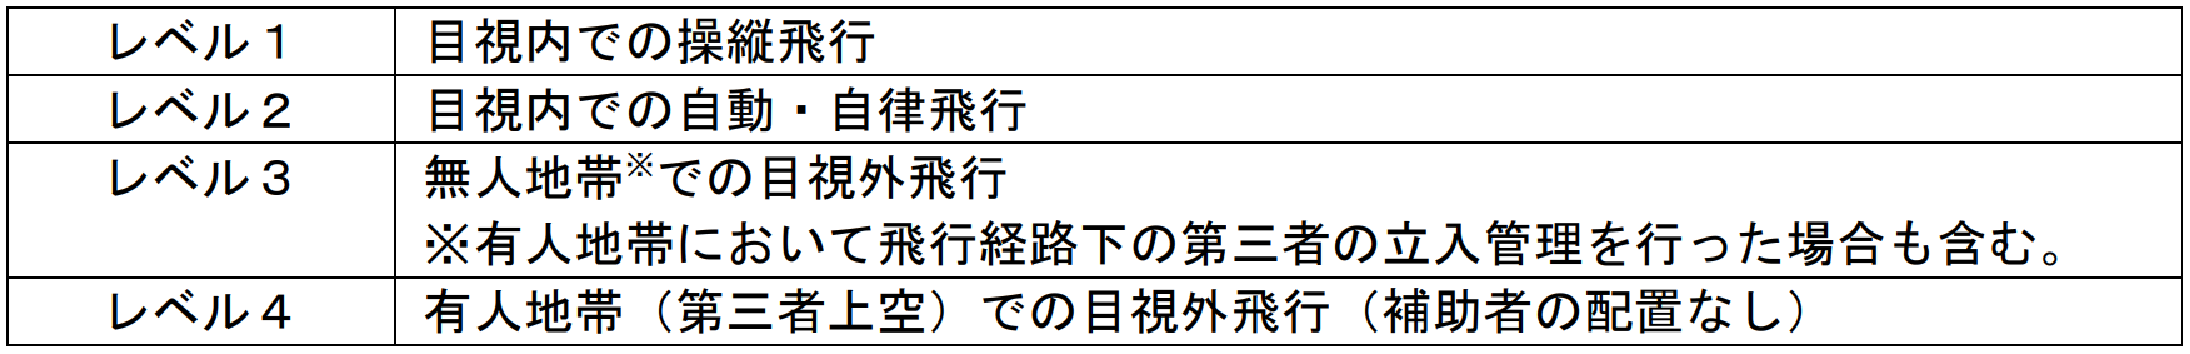
\includegraphics[width=0.8\textwidth]{flying_level.pdf}
  \label{fig:dron_level}
  \caption{ドローンの飛行レベル\cite{delivery_guidelines_2023}より引用}
\end{figure}

ドローン宅配をするにあたり該当するレベルは街中で事業者が事業所内で複数のドローンを管理することを想定しているためレベル4である.しかし,田畑が大部分の面積を占める地点や過疎地域の場合はレベル3に該当する可能性がある.

% 表\ref{tab:dron_level}のレベル4で定義されている「有人地帯での目視外飛行」が達成されるのであれば,定位置からドローンを飛ばし,ひとりの管理者で複数の場所にドローンを飛ばすことが可能となる.


\section{機能の概要・前提条件・制約事項}
\subsection{機能概要}
本システムは管理者,ドローン宅配事業者,使用者が存在する.それぞれに向けた機能の概要を説明する.
\subsubsection{管理者向け機能}
管理者用のwebページを作成し以下の機能を設ける.
\begin{description}[labelwidth=\linewidth]
  \setlength{\leftskip}{1em}
  \item [ログインログアウト機能]管理者がログインログアウトする機能.
  \item [利用者管理機能]利用者の登録情報の閲覧,絞り込み,請求書の送付,支払い状態の管理,アカウントの凍結を行う機能.
  \item [事業者管理機能]事業者の登録情報の閲覧,絞り込み,請求書の送付,支払う報酬額,支払い状態の管理,貸し出しドローン数,事業者の営業所情報,アカウントの凍結.
  \item [利用者情報分析機能]利用者の利用状況を絞り込みやグラフを用いて見る機能.
  \item [事業者情報分析機能]事業者の利用状況を絞り込みやグラフを用いて見る機能.
  \item [宅配依頼受付機能]利用者から宅配依頼を受け,受けることが可能か確認し,事業者に仕事を割り振ることが出来たら受付完了のフラグを返す機能 受付中,受付完了,集配中,配送中,配送完了くらいの状態を管理する.
  \item [宅配仕事割り振り機能]宅配依頼受付機能で呼び出す,事業者に仕事を割り振る機能,集配に向かう事業者と仲介トラックと最終的に配送する事業者の組み合わせを選ぶ.
  \item [ドローン貸出機能]事業者からドローンの貸出申請を受けて貸出あるいは,申請の差し戻しを行う機能.
  \item [事業者ドローン情報管理機能]事業者の所持ドローン,貸出用ドローンの登録,個数の変更,各ドローンの個体番号と稼働時間,状態の閲覧機能.
\end{description}

\subsubsection{事業者向け機能}
事業者用のwebページを作成し以下の機能を設ける.
\begin{description}[labelwidth=\linewidth]
  \setlength{\leftskip}{1em}
  \item [ログインログアウト機能] 事業者用のログインログアウト機能.
  \item [事業者登録申請] 事業者名,事業代表者,免許情報,口座情報,事業拠点,従業員数,電話番号,メールアドレス,施設情報,パスワードを入力して事業者登録申請を行う.
  \item [事業者情報編集機能] 事業者が登録している情報,事業者名,事業拠点数,事業所の場所,宅配事業規模,口座情報,代表者名,などを編集する機能.
  \item [依頼受注判断機能] 管理者から送られる宅配依頼を承諾もしくは拒否する機能.
  \item [配達完了通知機能] 宅配が完了した場合に利用者に通知する機能.
  \item [宅配場所登録機能] 宅配拠点を追加する機能.
  \item [使用ドローン登録機能] 事業者が独自に購入したドローンを登録する機能.
  \item [子アカウント発行機能] 権限を限定した一般従業員用アカウントを発行して,同一法人内で複数人が事業を行えるようにする機能.
  \item [ドローンレンタル機能] ドローンレンタルの申請をする機能.
  \item [退会機能] 事業者登録をやめて,退会をしてデータ削除を申請する機能.
\end{description}

\subsubsection{使用者向け機能}
使用者向けのAndroid端末ソフトウェアを用意し以下の機能を設ける.
\begin{description}[labelwidth=\linewidth]
  \setlength{\leftskip}{1em}
  \item [ログインログアウト機能] 使用者用のログインログアウト機能.
  \item [使用者会員登録機能] 使用者が会員登録をする機能,これは管理者の許可が必要ない.
  \item [宅配依頼機能] 宅配を依頼する機能.
  \item [宅配場所登録機能] 宅配で離着陸する場所を指定して登録する機能,外の画像を送信して申請をする.
  \item [お気に入り登録機能] 配送相手の住所と氏名をお気に入り登録する機能,これを用いて簡単に宅配を依頼する機能.
  \item [退会機能] 退会する機能.
\end{description}
\subsection{前提条件}
\begin{itemize}
  \item 宅配元と宅配先がお互いドローン着地地点を登録している
  \item 事業者は搬送装置を無人航空機の登録制度に基づき国土交通省のシステムに登録すること
  \item 宅配依頼に対し送り主と受け取り主の双方の同意している
  \item 利用者は日本語を理解できること
\end{itemize}
\subsection{制約条件}
\begin{itemize}
\item 利用者が情報を登録するときに虚偽の情報を登録しないこと
\item 管理者は利用者の情報を本システムの利用目的以外で使用しないこと
\item 管理者は利用者の個人情報の管理を情報漏洩のないように行うこと
\item 事業者は航空法施行規則236条に基づき搬送装置の適切な運用を行うこと
\item 荷物はW320$\times$D260$\times$H200(mm)以内に収まること\footnote{\label{fot:airtruck}物流専用ドローン AirTruck\cite{aeronext_airtruck}を想定}
\item 荷物は段ボールに梱包されていること
\item 荷物の重量は5kg以下であること\footref{fot:airtruck}
\item 利用者は利用規約を順守すること
\end{itemize}
\section{ドローン宅配・情報・金銭の流れ}

\subsection{ドローン宅配の流れ}
本システムで想定するドローン宅配の流れを図\ref{fig:overview_flow}に示す.
また,以下に詳細な流れを示す.

\begin{enumerate}
\item 送り主である利用者が,管理者に対して宅配依頼を行う.
\item 管理者が事業者に対し,集荷・配送依頼を行う.
\item 事業者がドローンを用い,依頼を受けた荷物の集荷を行う.
\item 受け取り主である利用者が事業者から離れている場合,トラックを用いて荷物を受け取り主の最寄りの事業者へ配送する.
\item 事業者がドローンを用い,荷物を受け取り主へ配達する.
\end{enumerate}

\begin{figure}[H]
  \centering
  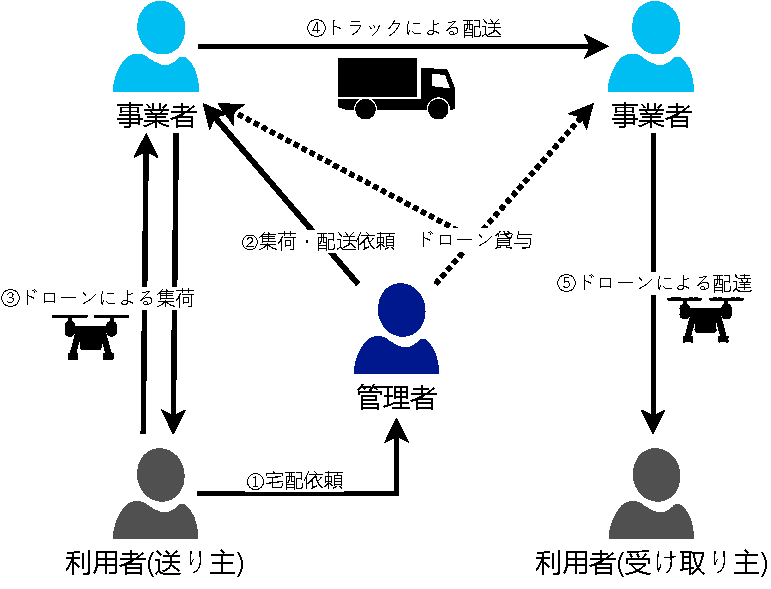
\includegraphics[width=0.6\linewidth]{./overview_flow.pdf}
  \caption{ドローン宅配の流れ}
  \label{fig:overview_flow}
\end{figure}

\subsection{情報の流れ}
本システムにおける情報の流れを図\ref{fig:info_flow}に示す.
本システムは,利用者(送り主及び受け取り主)が使用する端末,事業者が利用する端末,システム管理者が利用する端末及び,システム中核を担うサーバとデータベースによって構成される.

各ユーザからの要求を受けサーバが処理を行い,webページやアプリケーションに適した情報を提供する.

\begin{figure}[H]
  \centering
  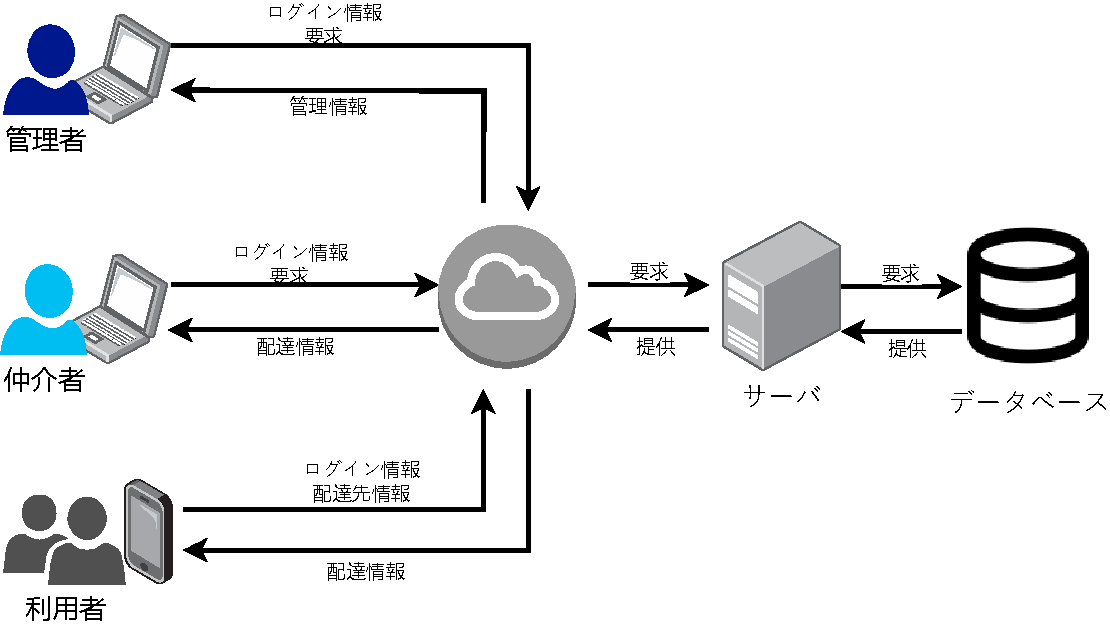
\includegraphics[width=0.6\linewidth]{./info_flow.pdf}
  \caption{本システムにおける情報の流れ}
  \label{fig:info_flow}
\end{figure}

\subsection{金銭の流れ}
本システムにおける金銭の流れを図\ref{fig:money_flow}に示す.

\begin{figure}[H]
  \centering
  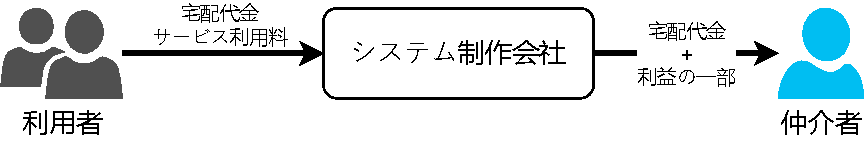
\includegraphics[width=0.6\linewidth]{./money_flow.pdf}
  \caption{本システムにおける金銭の流れ}
  \label{fig:money_flow}
\end{figure}


\section{想定する利用者}
本システムが想定する利用者を下記に示す.
\begin{itemize}
  \item 荷物の送受を希望する事業者または個人
  \item ドローン宅配事業者
\end{itemize}

\section{運用・保守}
\begin{itemize}
  \item ドローンを管理会社に委託する.
  \item サーバやシステムは自社が管理する.
  \item バグの修正を行う.
  \item システムのアップデートを行う.
  \item 不具合等の対応はメールまたは電話で対応する. 対応時間については表\ref{tb:huguai}に示す.
\end{itemize}

\begin{table}[htbp]
  \centering
  \begin{tabular}{c|c} \hline
    方法  & 対応時間          \\ \hline
    メール & 9:00 - 17:00  \\
    電話  & 10:00 - 15:00 \\ \hline
  \end{tabular}
  \caption{不具合等の対応時間}
  \label{tb:huguai}
\end{table}

\section{ハードウェア・ソフトウェアの構成}
\subsection{ハードウェア構成}
本システムのハードウェア構成を表\ref{fig:hardware}に示す.
\begin{table}[H]
  \begin{center}
    \caption{ハードウェアの構成}
    \label{fig:hardware}
    \begin{tabular}{ccc} \hline
      項目        & 種類      & 数量       \\ \hline \hline
      メインサーバ    & レンタルサーバ & 2        \\
      データベースサーバ & レンタルサーバ & 2        \\
      管理者端末     & PC      & 1        \\
      事業者端末     & PC      & 事業者数     \\
      利用者端末     & スマートフォン & 利用者数     \\
      搬送装置      & ドローン    & 事業者希望数以上 \\ \hline
    \end{tabular}
  \end{center}
\end{table}
\subsection{ソフトウェア構成}
本システムのソフトウェア構成を表\ref{fig:software}に示す.
\begin{table}[H]
  \begin{center}
    \caption{ソフトウェアの構成}
    \label{fig:software}
    \begin{tabular}{ccc} \hline
      項目           & ソフトウェア & 備考     \\ \hline \hline
      サーバ       & Webサーバ  &        \\
      サーバ & DBMS  &        \\
      管理者端末        & 管理者用システム &   \\
      事業者端末        & 事業者用システム &         \\
      利用者端末        & 利用者用システム & \\
      搬送装置         & ドローン管理システム &         \\ \hline
    \end{tabular}
  \end{center}
\end{table}

\section{費用・効果}
\subsection{システムの効果}
本システムを導入することによって,以下の効果が得られると考えられる.
\begin{itemize}
  \item ドローンを用いた無人宅配が可能となり,宅配サービスの人手不足を解消できる.
  \item ドローンを用いて処方薬を宅配することで,山間部や離島などに向けたリモート診療に利用できる.
  \item ドローンを用いた買い物代行やフードデリバリーといった新たなサービスが提供でき,経済の活性化につながる.
  \item 電動または電池駆動のドローンを使用することで,排ガス排出が削減され,環境への負荷が軽減する.
        そのため,環境への配慮を重視する現代社会に貢献できる.
\end{itemize}

\subsection{収益}
本システムの収益は配達による収入を想定している.配送料を600円,1日に配達する荷物の数を,宅配便の1日当たりの荷物数の約0.14\%の20,000個とすると5年間の配達による収入は
\begin{center}
  600円×20,000個×30日×60ヶ月=21,600,000,000円
\end{center}
となる.

\subsection{システムの導入・運用コスト}
本システムの導入コストは表\ref{tab:label1},運用コストは表\ref{tab:label2}のようになる.
\begin{table}[H]
  \centering
  \caption{導入コスト}
  \begin{tabular}{c c c c c}
    \hline
    項目          & 単価(円)     & 数量     & 金額(円)       & 備考 \\
    \hline \hline
    物流ドローン(貸出用) & 3,000,000 & 200台   & 600,000,000 &    \\
    サーバ(レンタル)   & 2,000     & 4ヶ月×2台 & 16,000      &    \\
    システム設計人件費   & 40,000    & 38日×2人 & 3,040,000   &    \\
    システム実装人件費   & 40,000    & 34日×6人 & 8,160,000   &    \\
    \hline \hline
                & 合計        &        & 612,736,000 &    \\
    \hline
  \end{tabular}
  \label{tab:label1}
\end{table}

\begin{table}[H]
  \centering
  \caption{運用コスト}
  \begin{tabular}{c c c c c}
    \hline
    項目        & 単価(円)       & 数量               & 金額(円)         & 備考               \\
    \hline \hline
    サーバ(レンタル) & 2,000       & 60ヶ月×2台          & 240,000       & 12ヶ月×5年×1台       \\
    維持費用      & 612,736,000 & 5年               & 306,368,000   & (導入コスト×10\% )×5年 \\
    宅配事業者報酬   & 150         & 20,000個×30日×60ヶ月 & 5,400,000,000 & 報酬×1日当たりの荷物の数×日数 \\
    中間配送費用    & 35000       & 40台×30日×60ヶ月     & 2,520,000,000 & 1台あたりの報酬×台数×日数   \\
    \hline \hline
              & 合計          &                  & 8,226,608,000 &                  \\
    \hline
  \end{tabular}
  \label{tab:label2}
\end{table}

上記を踏まえて,システムの開発と5年間の運用にかかる費用は次のようになる.
\begin{center}
  612,736,000円(導入コスト)+8,226,608,000円(運用コスト)=8,839,344,000円
\end{center}

\subsection{利益}
本システムを5年間運用した際の利益は以下のようになる.
\begin{center}
  21,600,000,000円(収益)-8,839,344,000(費用)=12,760,656,000円
\end{center}

\section{開発体制と工程計画}
本システムの開発は土佐山田IT株式会社の6名により実装する.

本システムの工程計画は図\ref{fig:schedule}に示す.
\begin{figure}[htbp]
  \label{fig:schedule}
  \centering
  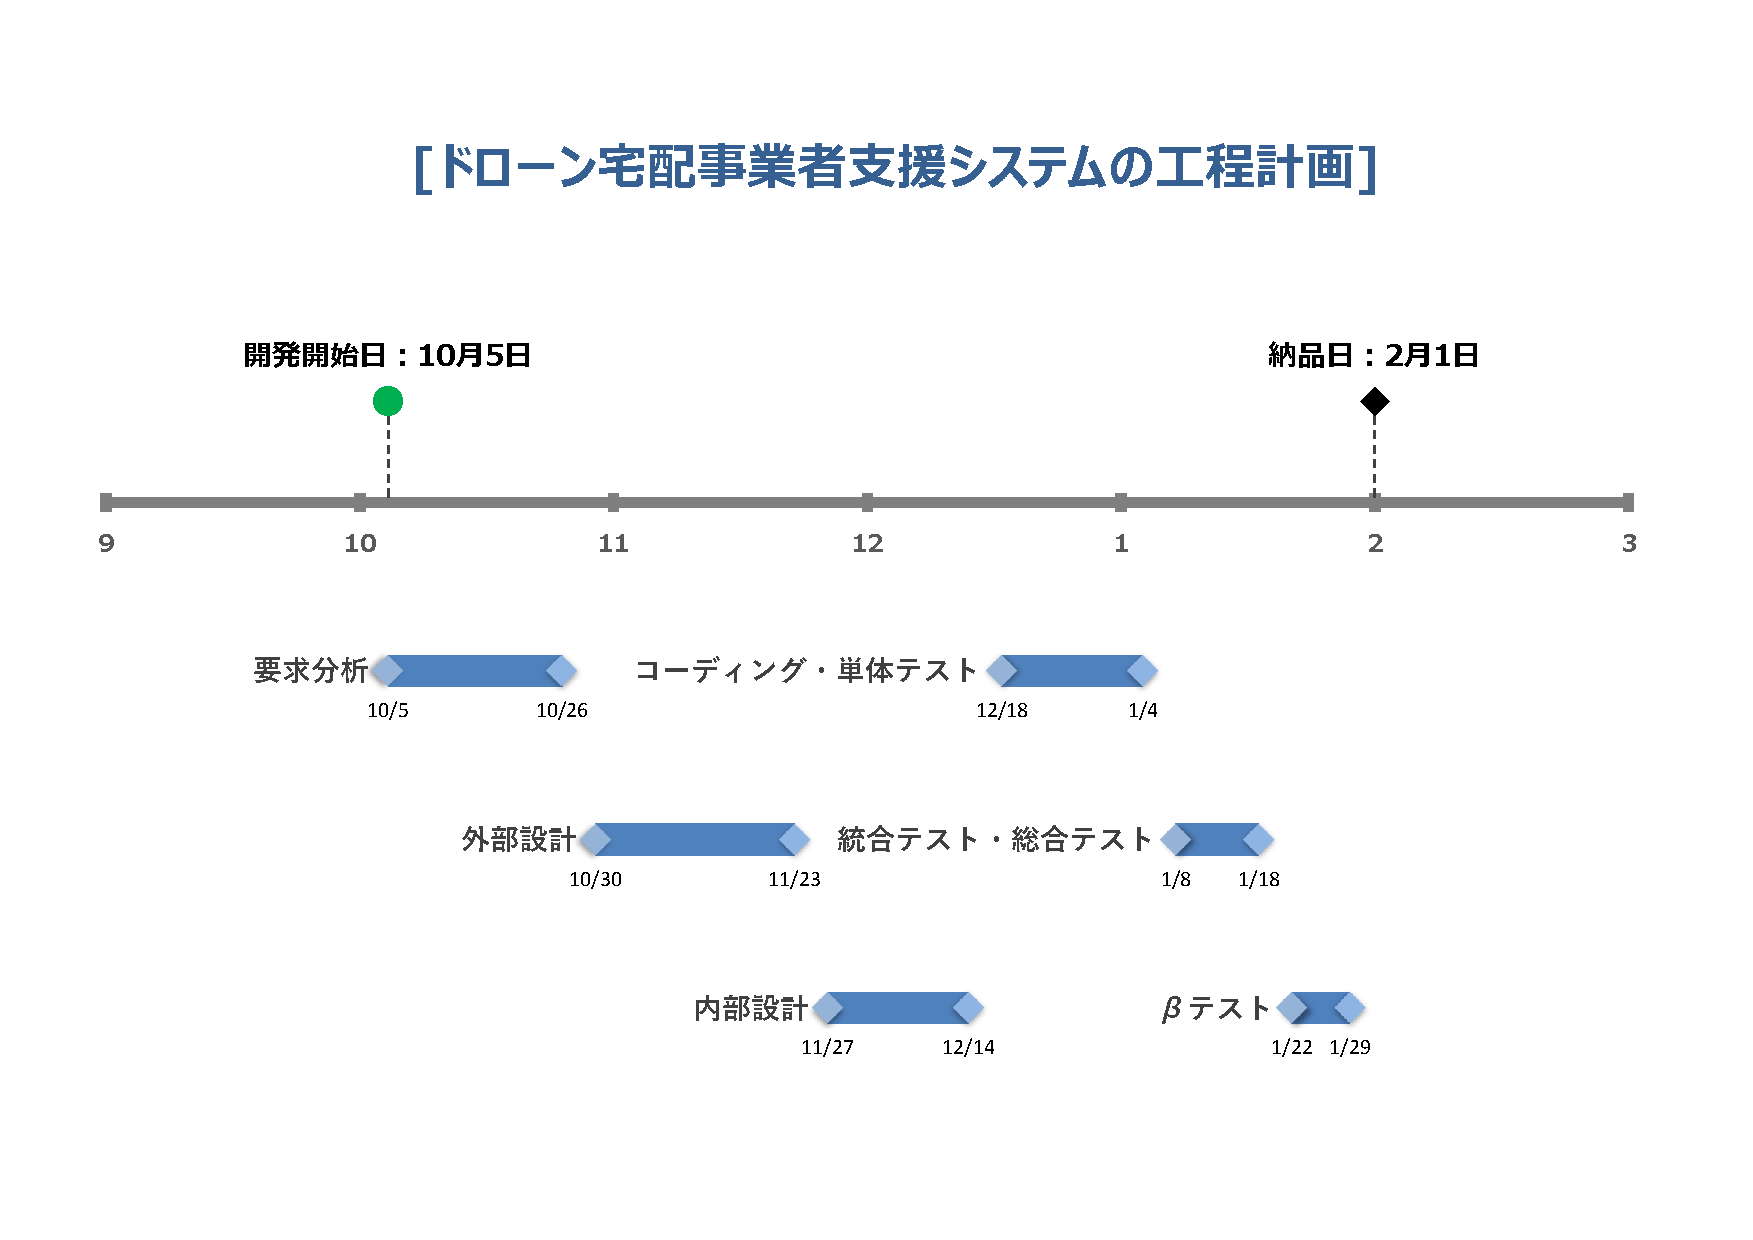
\includegraphics[width=0.8\textwidth]{schedule.pdf}
  \caption{工程計画}
\end{figure}

\section{本システムのアピールポイント}
\begin{enumerate}
  \item 未だに日本に存在のしないシステムである.
  \item 22年度の宅配荷物数は50億個であり,8年連続史上最高を更新中である.しかし,人手不足が深刻化しており,この課題の解決策のひとつとなりうる.
  \item 交通渋滞や地理的な制約を受けずに荷物を迅速かつ効率的に配達することが可能である.
  \item 災害時などで交通インフラが破壊されたとしても物理的障害の影響が少ないため,必要な物資や医療用品の迅速な配達が可能である.
  \item 離島や山間部などのアクセスが難しい地域において従来の宅配方法と比較し,大幅なコスト削減になる.
  \item 今日リモート診療が普及し始めている.リモート診療とドローン宅配を併用すると患者は外出する必要がなくなるため,感染リスクを極力減らすことができる.
\end{enumerate}

\section{貢献度}
システム提案書では各メンバーが以下を担当した.
\begin{enumerate}
  \item 1240312 久保田 天治: 機能の概要・前提条件・制約事項一部,ハードウェアとソフトウェアの構成
  \item 1250329 塩澤 康志: 費用・効果
  \item 1250333 蝉 祐介: 運用・保守
  \item 1250348 寺内 俊輔: 機能の概要・前提条件・制約事項一部,現状の課題,課題解決のための提案,全体の枠組み,全体の統合
  \item 1250358 林 晃太郎: 想定する利用者,スケジュール,本システムのアピールポイント
  \item 1250371 松本 吏司: 情報・金銭の流れ,全体の枠組み
\end{enumerate}

\bibliography{References.bib}
\bibliographystyle{plain}


\end{document}
